\documentclass[FinalReport.tex]{subfiles}

\begin{document}
Consider a one dimensional time-discrete random map 

\begin{equation}\label{eq:uncontrolled}
	y_{t+1}=\alpha_0y_t + \beta_t,	
\end{equation}
where the dynamical variable $y_t$ denotes the deviation of a system from some target value at time $t$ ($t=0,1,\dots$). $\alpha_0$ is a system parameter unknown to the controller and assumed to be a constant larger than $1$, therefore making the system unstable. $\beta_t\sim\mathcal{N}(0,\sigma_0^2)$ is a Gaussian random variable describing non-predictable fluctuations; its variance $\sigma_0^2=\text{const}$ is a second hidden parameter.
%% TODO : check typos (see comment) 

The controller is assumed to know the form of the dynamical equation \eqref{eq:uncontrolled}. A control strategy consists in computing an estimate $\hat{\alpha}_0^{(n)}$ of $\alpha_0$ from $y_t$ and $n$ previous observations $y_{t-1},y_{t-2},\dots y_{t-n}$. At each time step the controller removes the predicted deviation $c_ty_t$ to the dynamics \eqref{eq:uncontrolled}, with $c_t=\hat{\alpha}_0^{(n)}$. When control is switched on, the map is replaced by
\begin{equation}\label{eq:map}
	z_{t+1}=(\alpha_0-c_t)z_t+\beta_t,	
\end{equation}
where $z_t$ denotes the controlled dynamics. Control is said optimal if controlled dynamics \eqref{eq:map} follows noise distribution.

Estimates $\hat{\alpha}_0^{(n)}$ are be obtained by Maximum Likelihood Estimation (MLE), as in \cite{OptCont}. The likelihood is the joint probability of observing $z_t$ and the past realizations $\{z_{t-i-1}\}_{i=0}^{n-1}$ given $\{c_{t-i-1}\}_{i=0}^{n-1}\equiv c_i^n$, as a function of $\alpha_0$:
\begin{align}
	\mathcal{L}(\{z_{t-i-1}\}_{i=0}^{n-1};\alpha_0,c_i^n)&\equiv P(z_t,z_{t-1},\dots,z_{t-n}\vert \alpha_0;c_i^n)\label{eq:mle}.
\end{align}
Iterating Bayes' law gives
\begin{equation}
	\mathcal{L}(\{z_{t-i-1}\}_{i=0}^{n};\alpha_0,c_i^n)=\prod_{i=0}^{n-1}P(z_{t-i}\vert z_{t-i-1},\dots z_{t-n};\alpha_0,c_i^n) P(z_{t-n}\vert \alpha_0;c_i^n),
\end{equation}
and the log likelihood is
\begin{equation}\label{eq:log_lik_full}
	l(\{z_{t-i-1}\}_{i=0}^{n};\alpha_0,c_i^n)=\sum_{i=0}^{n-1}\log\bigl(P(z_{t-i}\vert z_{t-i-1},\dots z_{t-n};\alpha_0,c_i^n)\bigr) + \log\bigl(P(z_{t-n}\vert \alpha_0;c_i^n)\bigr).
\end{equation}
Next we drop the last term by assuming that without knowing previous deviations, distribution of $z_{t-n}$ is independent of $\alpha_0$: $\partial_{\alpha_0}{P(z_{t-n}\vert \alpha_0;c_i^n)}=0$. Indeed, without knowledge of the starting point $z_{t-1}$, $z_t$ could be anywhere, irrespective of $\alpha_0$ and $c_{t-1}$ (this assumption is numerically validated in \cite{OptCont}). The estimator of $\alpha_0$ is then
\begin{equation}\label{eq:log_like}
	\hat{\alpha}_0^{(n)}=\argmax_{\alpha_0}\sum_{i=0}^{n-1}\log(P(z_{t-i}\vert z_{t-i-1},\dots z_{t-n};\alpha_0,c_i^n)).
\end{equation}
Given \eqref{eq:map}, the dynamic is conditionally Gaussian:
\begin{equation}
	P(z_{t-i}\vert z_{t-i-1},\dots z_{t-n},\alpha_0;c_i^n)=\frac{1}{\sqrt{2\pi\sigma_0^2}}e^{-\frac{1}{2\sigma_0^2}\bigl(z_{t-i}-(\alpha_0-c_{t-i-1})z_{t-i-1}\bigr)^2}.
\end{equation}
Plugging into \eqref{eq:log_like}:
\begin{equation}
\hat{\alpha}_0^{(n)}=\argmin_{\alpha_0}\left[\frac{1}{2\sigma_0^2}\sum_{i=0}^{n-1}\bigl(z_{t-i}-(\alpha_0-c_{t-i-1})z_{t-i-1}\bigr)^2 +\frac{1}{2}\log(2\pi\sigma_0^2)\right].
\end{equation}
The first order condition reads
\begin{equation}
0=\left.\pdv{}{\alpha_0}\right\vert_{\hat{\alpha}_0^{(n)}}\log(P(z_{t-i}\vert z_{t-i-1},\dots z_{t-n};\alpha_0,c_i^n))=\frac{1}{\sigma_0^2} \sum_{i=0}^{n-1} z_{t-i-1}z_{t-i}-\alpha_0z_{t-i-1}^2+c_{t-i-1}z_{t-i-1}^2,
\end{equation}
and finally the estimator is 
\begin{equation}\label{eq:controller_mle_n}
	\hat{\alpha}_0^{(n)}=\frac{\sum_{i=0}^{n-1}c_{t-i-1}z_{t-i-1}^2+z_{t-i-1}z_{t-i}}{\sum_{i=0}^{n-1}z_{t-i-1}^2}.
\end{equation}
MLE estimator is asymptotically normal \cite{CoxHink74}: $(\hat{\alpha}_0^{(n)}-\alpha_0)\underset{n\rightarrow\infty}{\stackrel{d}{\longrightarrow}}\mathcal{N}\left(0,\frac{1}{n}\mathcal{I}^{-1}\right)$, where 
\begin{equation}\label{eq:MLE_var}
	 \mathcal{I}=\mathbb{E}[-\partial^2_{\alpha_0}\vert_{\hat{\alpha}_0^{(n)}} \log\bigl(P(z_{t-i}\vert z_{t-i-1},\dots z_{t-n};\alpha_0,c_i^n)\bigr)]=\frac{1}{\sigma_0^2}\expval{\sum_{i=0}^{n-1}z^2_{t-i-1}}
\end{equation} 
is the Fischer information. It measures the amount of information that $\{z_{t-i-1}\}_{i=0}^{n}$ carries about $\alpha_0$. The variance of $\hat{\alpha}_0^{(n)}$ (see \autoref{app:var_a0} for a more detailed derivation) is then
\begin{equation}\label{eq:MLE_var}
	s_n^2=\frac{\sigma_0^2}{n^2\expval{\sum_{i=0}^{n-1}z^2_{t-i-1}}}.
\end{equation}
When $n$ is sufficiently large, $\E{z_t^2}$ is well defined such that \eqref{eq:MLE_var} becomes $s_n^2=\sigma_0^2/(n^2 \hat{\sigma}_z^2)$ and
vanishes with $n$. Fluctuations of long memory systems are then normally distributed, with variance $\sigma_0^2$:
\begin{equation}
	z_{t+1}\equiv(\alpha_0-c_t)z_t+\beta \widesim{n\gg 1} \mathcal{N}\left(0,\sigma_0^2 \right).
\end{equation}

%%%%%%%%%%%%%%%%% n=50 stats %%%%%%%%%%%%%%%%%%%%%
\def\longz{8.74}
\def\explongz{-4}
\def\longvarz{0.81}
\def\longmaxz{0}


\section{Numerical results}
Numerical solution off $P(z_t)$ for $n=50$ approaches noise (Figure \ref{fig:dist_n_large}), with $\expval{z_t}=\longz\cdot10^{\explongz}$ and $\expval{z_t^2}=\longvarz$. To test Goodness-of-Fit we compute first the Kolmogorov-Smirnov (KS) statistics \cite{stat_meth}, which tests the null hypothesis that 
$z_t\sim\N(0,\sigma_0^2)$. With the numerical solution, KS statistics is $1.19\cdot10^{-3}$ with $p-$value 0.53. The null hypothesis is therefore acceptable. We also present results from Anderson-Darling test gives more weight to the tail \cite{test_comp}, which is relevant in our case. The simulation yields a critical value $D=0.441$, inferior to the critical value with significance level $15\%$ for a normal distribution, $0.576$ \cite{anderson-test}. Again, normality assumption is accepted.
\begin{figure}[h]
	\centering
	\makebox[\textwidth][c]{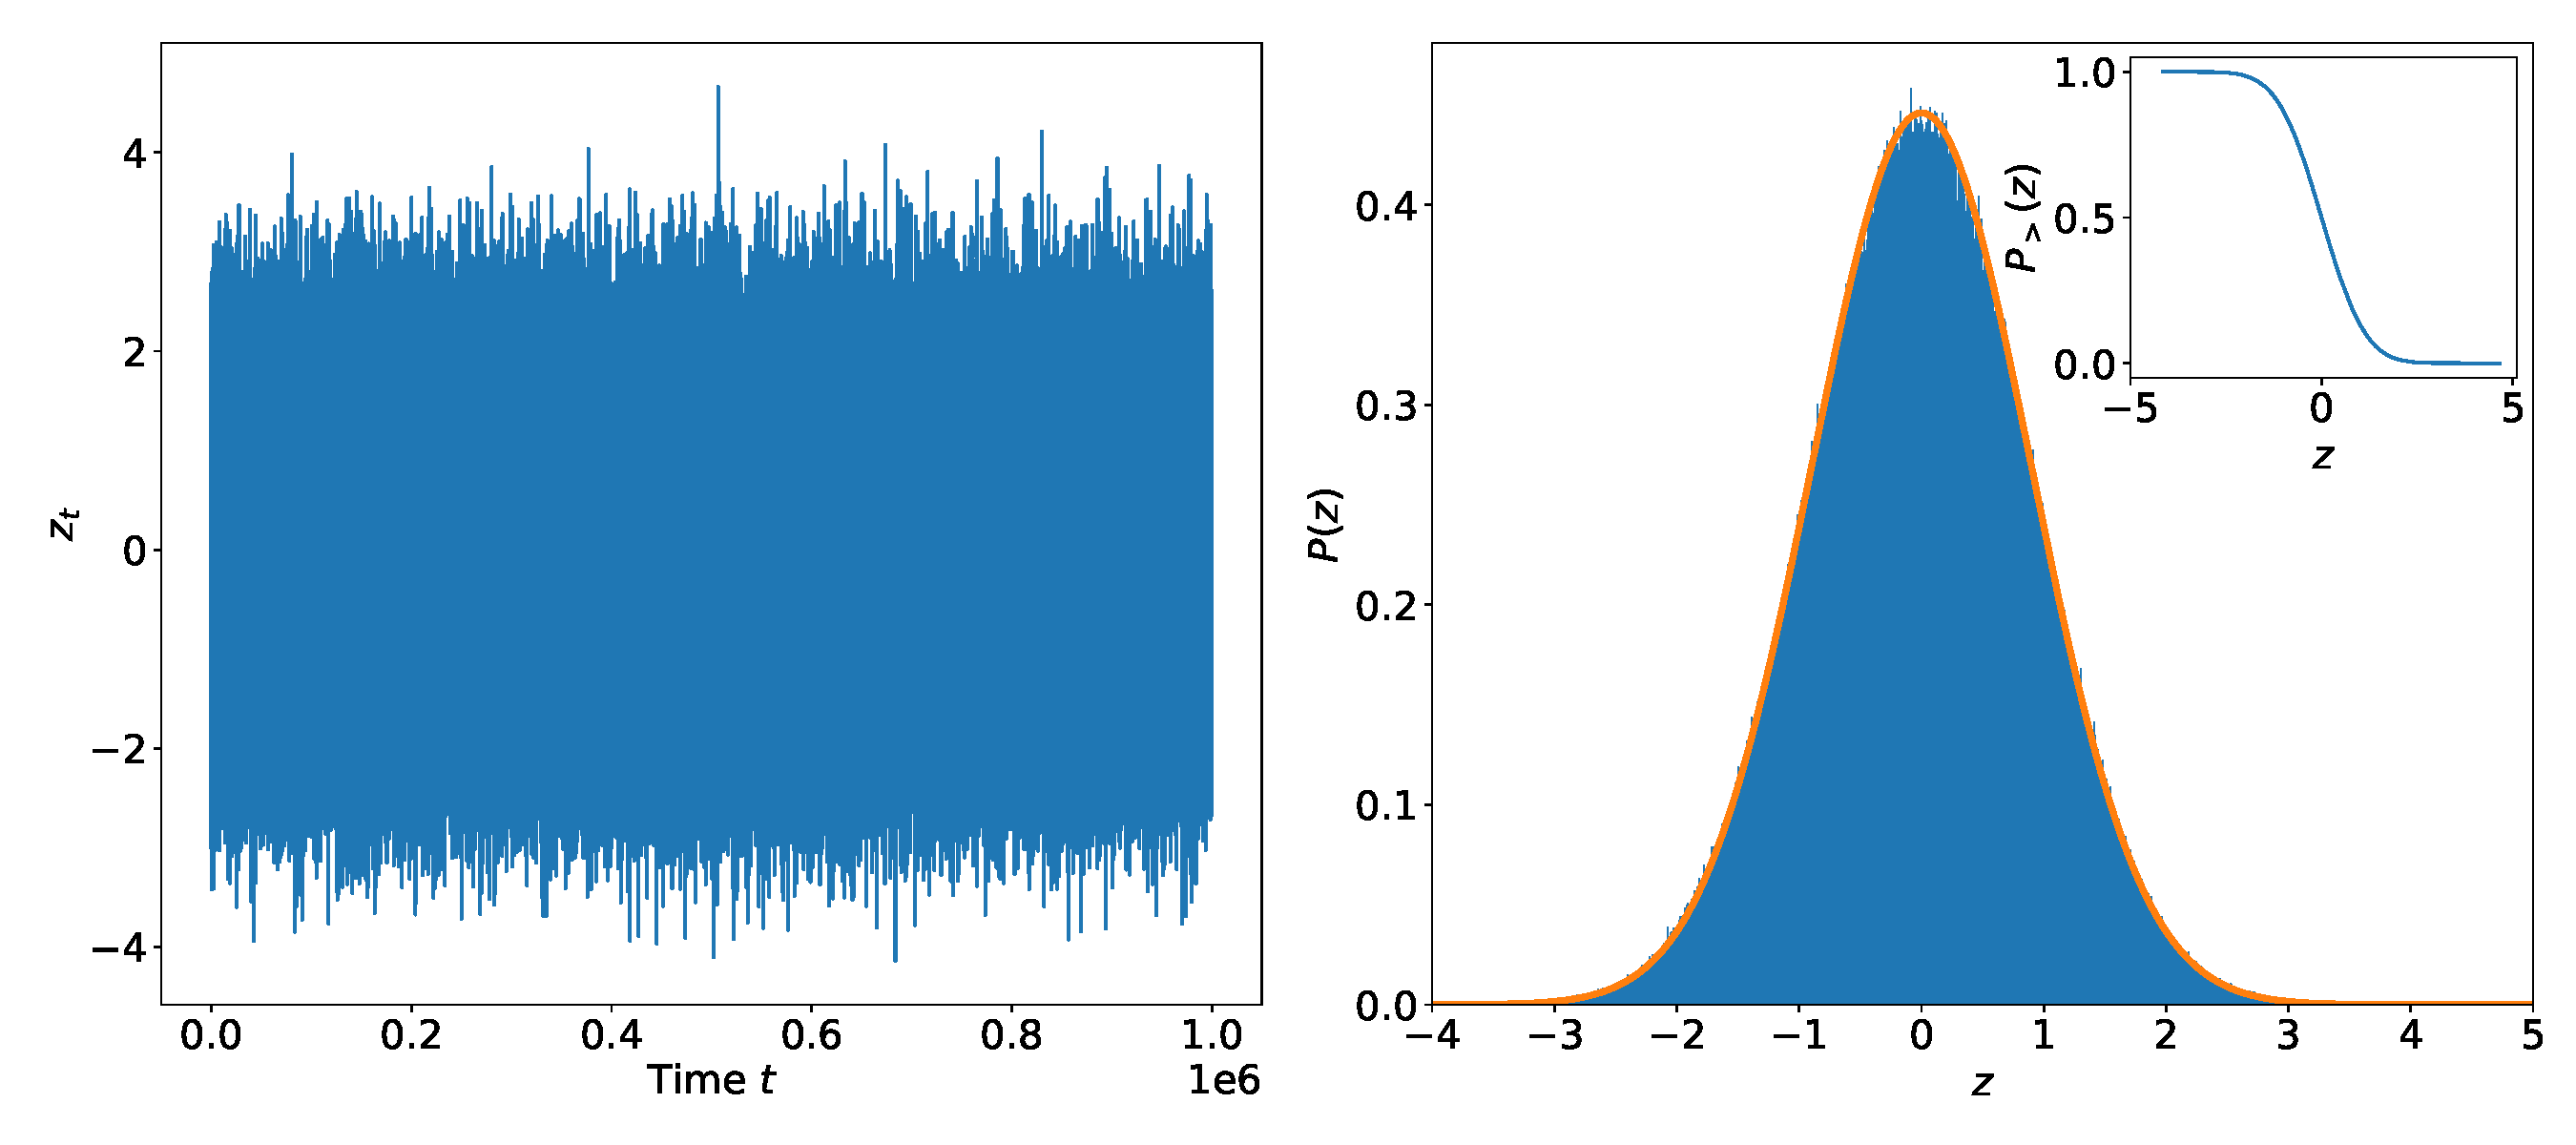
\includegraphics[width=1.1\textwidth,scale=1]{Graphs/dist_n=50.pdf}}		
	\caption{Left: solution of \eqref{eq:map} with controller \eqref{eq:controller_mle_n} and $n=50$ look-backs. Right: associated histogram, compared with $P_\beta\sim\mathcal{N}(0,\sigma_0^2)$ (orange) and complementary cumulative distribution function (CCDF, inset). $N=10^6$ time-steps, $\alpha_0=2$, $\sigma_0^2=0.8$, $z_0=1$. $\expval{z}=\longz\cdot10{\explongz}$ and $\expval{z^2}=\longvarz$.}
	\label{fig:dist_n_large}
\end{figure}

%%%%%%%%%%%%%%%%% n=1 stats %%%%%%%%%%%%%%%%%%%%%
\def\z{0.916}
\def\varz{5.89}
\def\varzexp{5}
\def\maxz{3.29}
\def\maxzexp{5}

For very small $n$, those properties are not guaranteed. The variance of the estimator \eqref{eq:MLE_var} $\sigma_0^2/(n^2\expval{z_t^2})$ diverges as $z_t\rightarrow0$ because Fischer information (knowledge about $\alpha_0$ in the past observations) decreases as control gets better. 
Trajectory $z_t$ simulated with $n=1$ (Figure \ref{fig:dist_n=1}) exhibits extreme deviations, with $\max_{t}\{z_t\}=\maxz\cdot10^{\maxzexp}$ while last percentile is $\Q(99\%)=54.52$. The difference between them enlightens the presence of a heavy tail. Even though $83.3\%$ of the fluctuations are within the expected range for a normal distribution, remaining tail dominates the statistics.
 Besides, the complementary cumulative distribution function (CCDF, Figure \ref{fig:dist_n=1}) demonstrate a power-tail with exponent $\mu=1$ as suggested in \cite{OptCont, FrontNanoScience}:
\begin{align}\label{eq:pt}
	P(z)=\frac{C}{z^{1+\mu}}, \quad P_>(z)=P(Z>z)=\frac{C}{z^\mu}.
\end{align}
where $P_>$ is the tail distribution or CCDF.
\begin{figure}[h!]
	\centering
	\makebox[\textwidth][c]{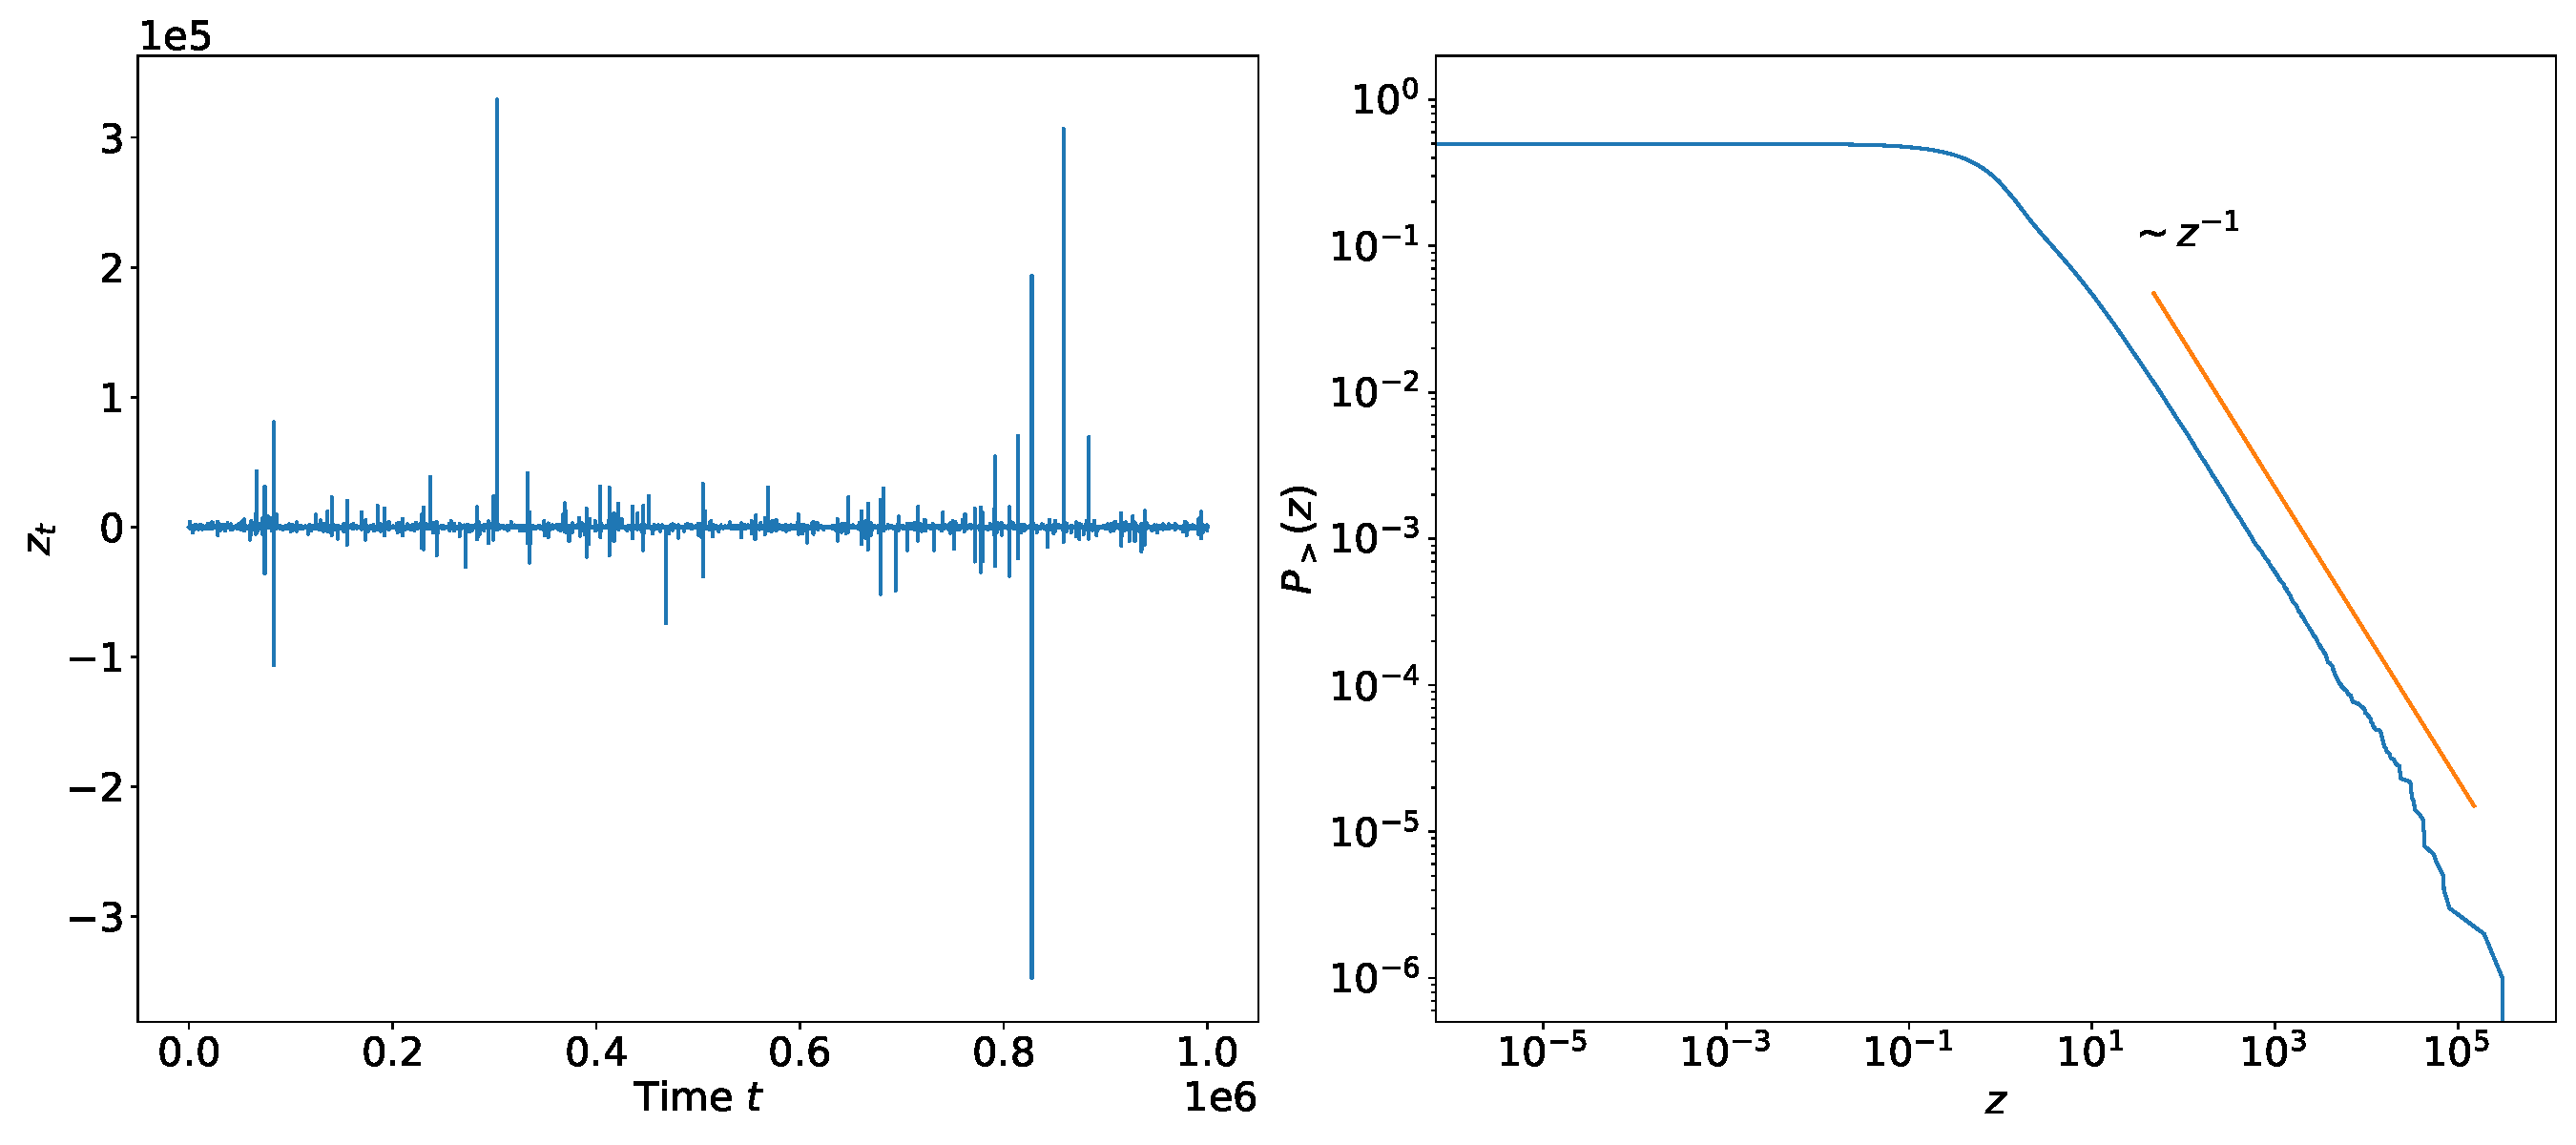
\includegraphics[width=1.1\textwidth,height=.43\textwidth]{Graphs/dist_n=1.pdf}}
	\caption{Left: solution of\eqref{eq:map} with controller \eqref{eq:controller_mle_n} and $n=1$ look-back. Right: log-log plot of CCDF $P_>(z)$ with reference line $z^{-1}$. $N=10^6$ time-steps, $\alpha_0=2$, $\sigma_0^2=0.8$, $z_0=1$.}
	\label{fig:dist_n=1}
\end{figure}

\section{Convergence of the tail}

This behavior comes from the estimation of $\alpha_0$ \eqref{eq:controller_mle_n}, which involves the sample variance in the denominator. In the case $n=1$ the dynamics reads
\begin{equation}\label{eq:dyn_n=1}
	z_{t+1}=\left(\alpha_0-c_{t-1}-\frac{z_t}{z_{t-1}} \right)z_t + \beta_t.	
\end{equation}
When the dynamics is well controlled the estimator $c_{t-1}$ is close to the ground truth $\alpha_0$ and $z_{t-1}$ is close to $0$. If besides $(\alpha_0-c_{t-1})z_{t-1}\sim\mathcal{O}(1)$, $z_t$ is also of order $1$ and thus $\frac{z_t}{z_{t-1}}$ diverges.
Using conservation of probability:
\begin{equation}
	P(z_{t+1})=P(z_{t-1})\abs{\frac{\dd{z_{t-1}}}{\dd{z_{t+1}}} }.
\end{equation}
Replacing $z_{t-1}=\frac{-z_t^2}{(z_{t+1}-\beta_t)-(\alpha_0-c_{t-1})z_t}\underset{z_{t+1}\gg1}{\longrightarrow}0$ and $\abs{\frac{\dd{z_{t-1}}}{\dd{z_{t+1}}} }=\frac{z_t^2}{[(z_{t+1}-\beta_t)-(\alpha_0-c_{t-1})z_t]^2}$, the tail of the distribution is
\begin{equation}\label{eq:tail_p(z)_n=1}
	P(z_{t+1})\propto \frac{1}{z_{t+1}^{2}}
\end{equation}
as $P(z_{t-1})$ becomes a constant when $z_{t-1}$ goes to\footnote{Power laws are constant below some threshold $z_m>0$.} $0$.
Control still works as $z_t$ stays bounded but is not optimal because of the heavy tailed time series, which generates large deviations and a divergent variance.
With larger $n$ the estimator \eqref{eq:controller_mle_n} gives better results, and the tail distribution $P_>(z_t)$ gets thinner. 

This estimator is a sum of random variables divided by the sample variance of $z$, which resembles the origin of a Student's $t-$distribution with $n$ degree of freedom \cite{CritPhenom}:
\begin{equation}
	f_n(x) = \frac{\Gamma(\frac{n+1}{2})} {\sqrt{n\pi}\,\Gamma(\frac{n}{2})} \left(1+\frac{x^2}{n} \right)^{\!-\frac{n+1}{2}},
\end{equation}
which has asymptotic tail $\abs{x}^{-(n+1)}$; fitting with the exponent $\mu^{(n)}=n$ obtained numerically Figure (\ref{fig:KL_n}) and suggested in \cite{OptCont}.




\begin{figure}[h!]
	\centering
	\makebox[\textwidth][c]{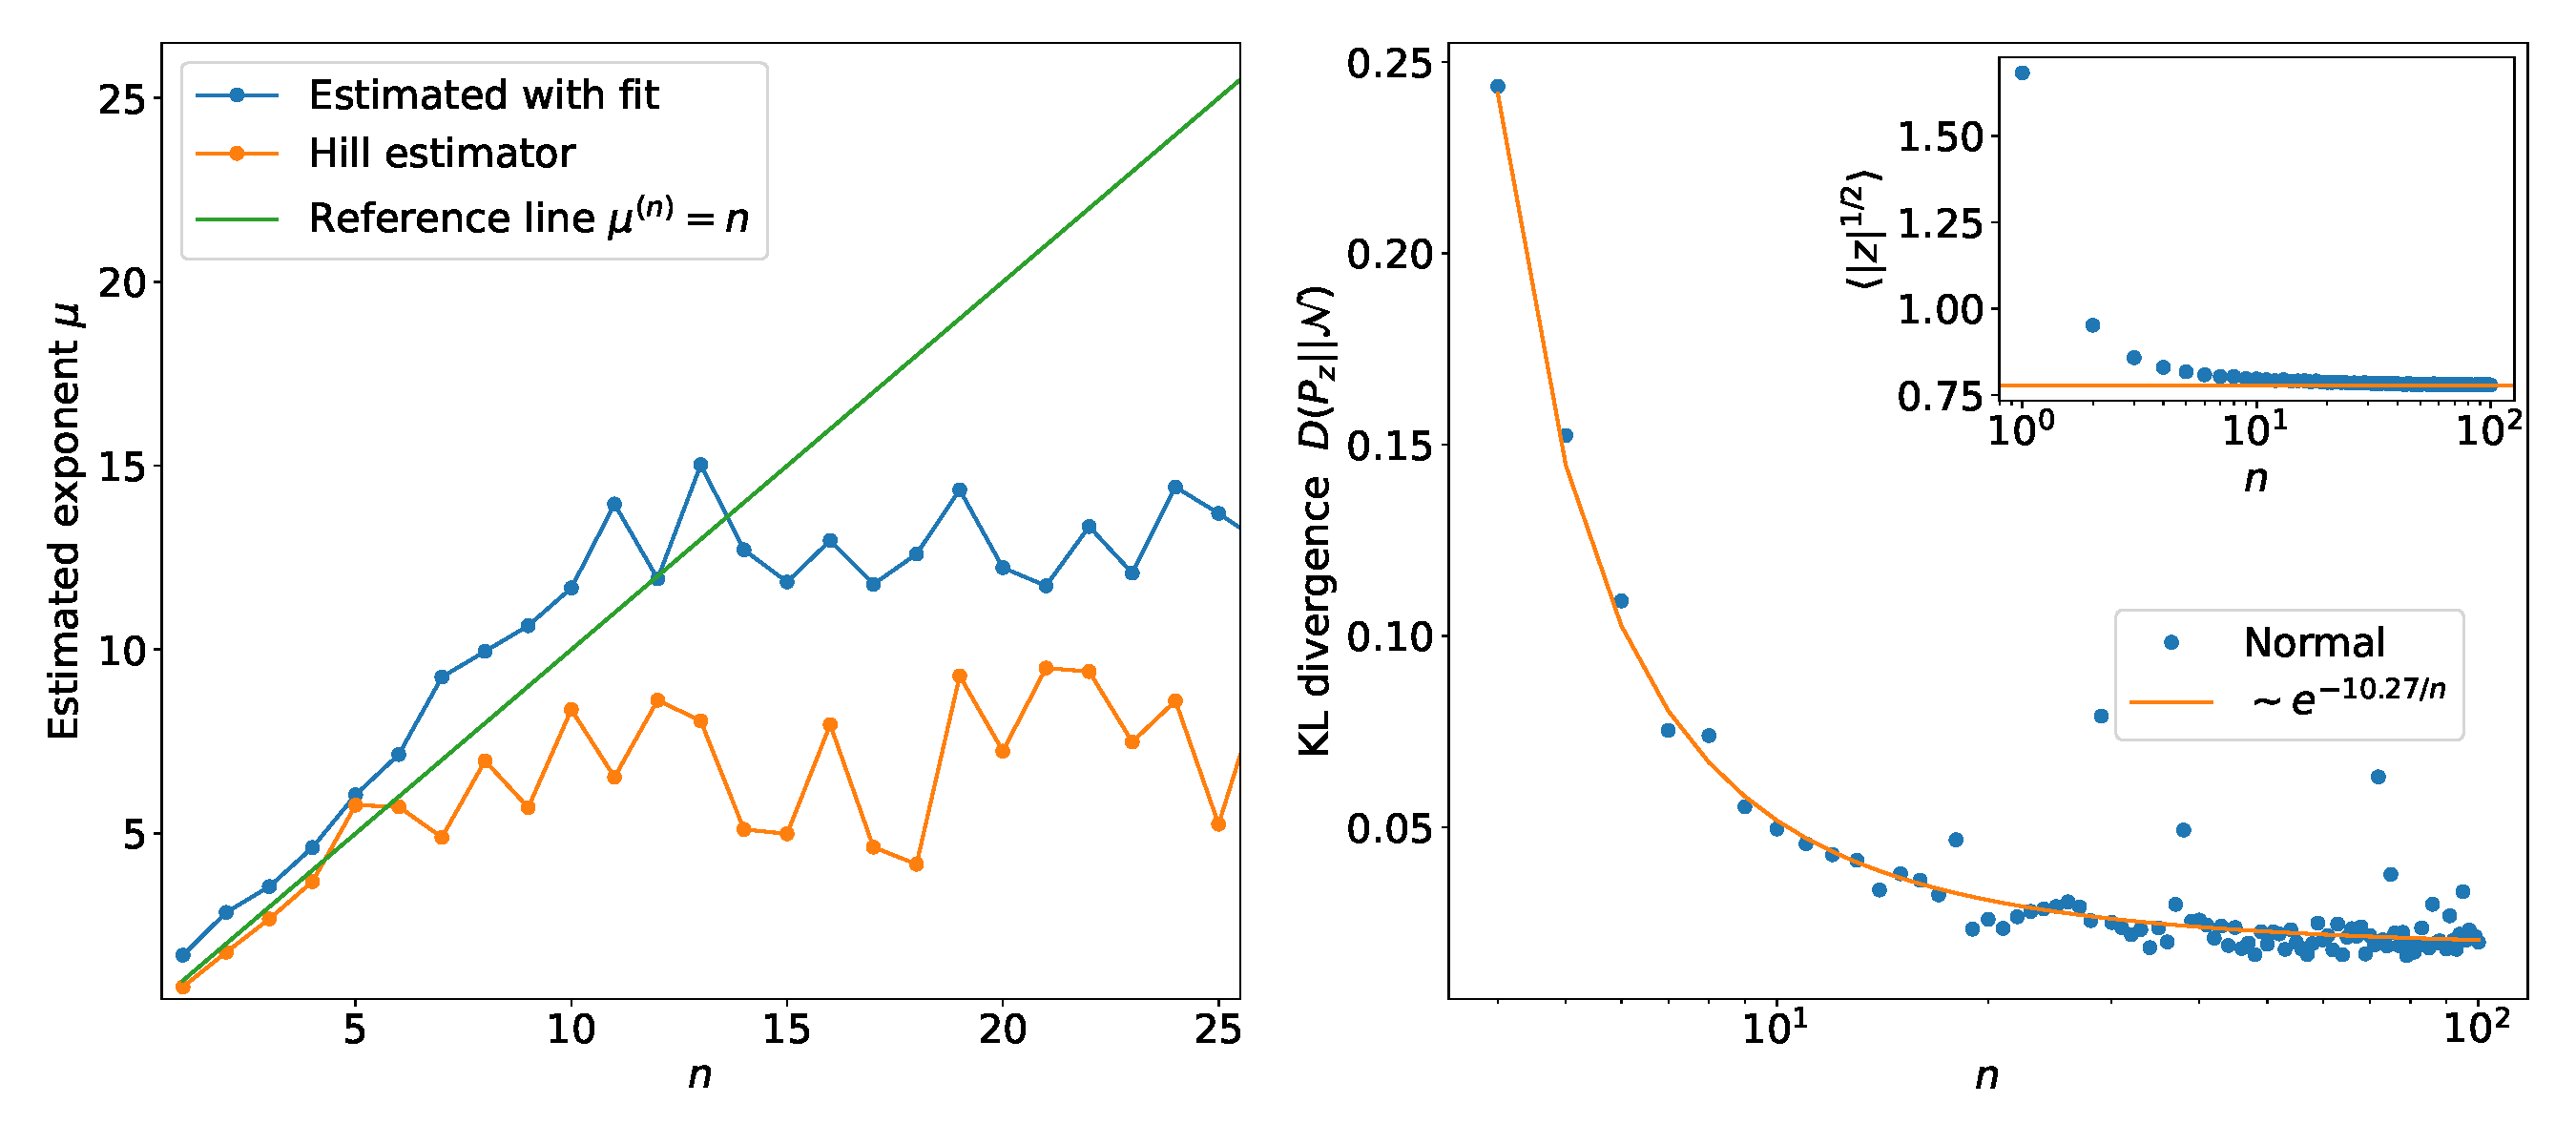
\includegraphics[width=1.1\textwidth,height=.43\textwidth]{Graphs/KL_n.pdf}}
	\caption{Left: Tail exponent for different $n$, obtained by fitting the CCDF (blue) or with Hill estimator (orange, \cite{Hill75}). Green line is the postulated exponent $\mu^{(n)}=n$ \cite{OptCont,FrontNanoScience}.
	Right: Convergence toward a Gaussian. Kullback-Leibler divergence between simulated distribution $P(z_t)$ and a centered normal distribution $\mathcal{N}(0,\sigma_0^2)$ (blue). In orange reference line $e^{-C/n}$ with $C\approx-10.27$, indicating a threshold at $n^*\approx 10$. After $n^*$ empirical distribution is close to the normal one, and adding more look-backs does not change the behavior. Inset: absolute half moment $\expval{\abs{z}^{1/2}}$ compared with theoretical value $\E{\abs{X}^{1/2}} \approx0.778$ (orange line) for $\mathcal{N}(0,\sigma_0^2)$. $N=10^5$ time-steps, $\alpha_0=2$, $\sigma_0^2=0.8$, $z_0=1$.}
	\label{fig:KL_n}
\end{figure} 


This asymptotic power law behavior is stable upon convolution with additive scaling factor \cite[chap.~4]{CritPhenom}. The tail of a sum of $n$ random variables following \eqref{eq:pt} with $\mu=n$ is thus distributed as  
\begin{equation}
	P_n(z)\sim \frac{n}{z^{1+\mu}}, \quad z\rightarrow\infty	
\end{equation}
However, if $\mu>2$ variance $\expval{z^2}$ is mathematically defined so the sequence converges to a Gaussian distribution with variance $n\expval{z^2}$. This convergence occurs for the centre of the pdf (small values) but is not guaranteed beyond a certain threshold, where it stays a power law \cite[chap.~3]{CritPhenom}. The threshold between those two regimes is obtained by matching distributions:
\begin{subequations}\label{eq:z0}
	\begin{align}
	P_n(z)&\sim \frac{1}{\sqrt{2\pi n}}e^{-\frac{z^2}{2n}}, \quad z<z_0\\
	P_n(z)&\sim \frac{n}{z^{1+\mu}}, \quad z>z_0.
	\end{align}
\end{subequations}

Equating them, one gets $z_0(n)\sim\sqrt{n\log{n}}$. If $z_{max}=\max_{t}\{z_t\}<z_0(n)$ then the time series exhibits no deviations outside of Gaussian regime. With power law distributed time series, the typical maximum after $N$ steps is $m_\mu\sim N^{1/\mu}$, while it is $m_\mathcal{N}\sim\sigma\sqrt{2\log(N)}$ for a normally distributed sequence (see  \autoref{app:max_distrib}). Numerical simulations indeed reveal two regimes for $z_{max}$ (Figure \ref{fig:max_exp_n}): for small $n$ it follows exactly the typical maximum of a power law distribution $m_\mu(n)$ with exponent $\mu^{(n)}=n$. But once the maximum deviation gets smaller than $z_0(n)$, $z_{max}$ becomes independent of $n$, equal to $m_\mathcal{N}\approx 4.27$ (for $N=10^5$). Figure \ref{fig:ccdf_n} gives CCDF for some values on $n$; highlighting the convergence towards a normal distribution.
Figure \ref{fig:KL_n} shows the Kullback-Leibler (KL) divergence between the empirical distribution and noise distribution $\mathcal{N}(0,\sigma_0^2)$ versus $n$. It decreases fast for small $n$ and stays constant close to $0$ for $n\gtrsim10$, implying that $z_t$ reaches its final distribution. 
Figure \ref{fig:KL_n} also shows the absolute half moment\footnote{Moments with $k\geq1$ are not defined for power laws with $\mu=1$ hence we use $k=1/2$ moment.} $\expval{\abs{z}^{1/2}}$ versus $n$, which tends to the theoretical value\footnote{$\mathbb{E}[\abs{X}^{1/2}]=\int \d x \frac{\abs{x}^{1/2}}{\sqrt{2\pi\sigma_0^2}}e^{-\frac{x^2}{2\sigma_0^2}}=\sqrt{\frac{\sigma_0\sqrt{2}}{\pi}}\Gamma\left(\frac{3}{4}\right)\approx 0.778$ for $\sigma_0^2=0.8$.} at $n\gtrsim 10$. For $N=10^5$, the maximum of the normal distribution $m_\mathcal{N}$ equals $z_0(n)$ for $n\approx 8.57$, justifying the change of regime observed Figure \ref{fig:max_exp_n}.
\begin{figure}[h!]
	\centering
	\makebox[\textwidth][c]{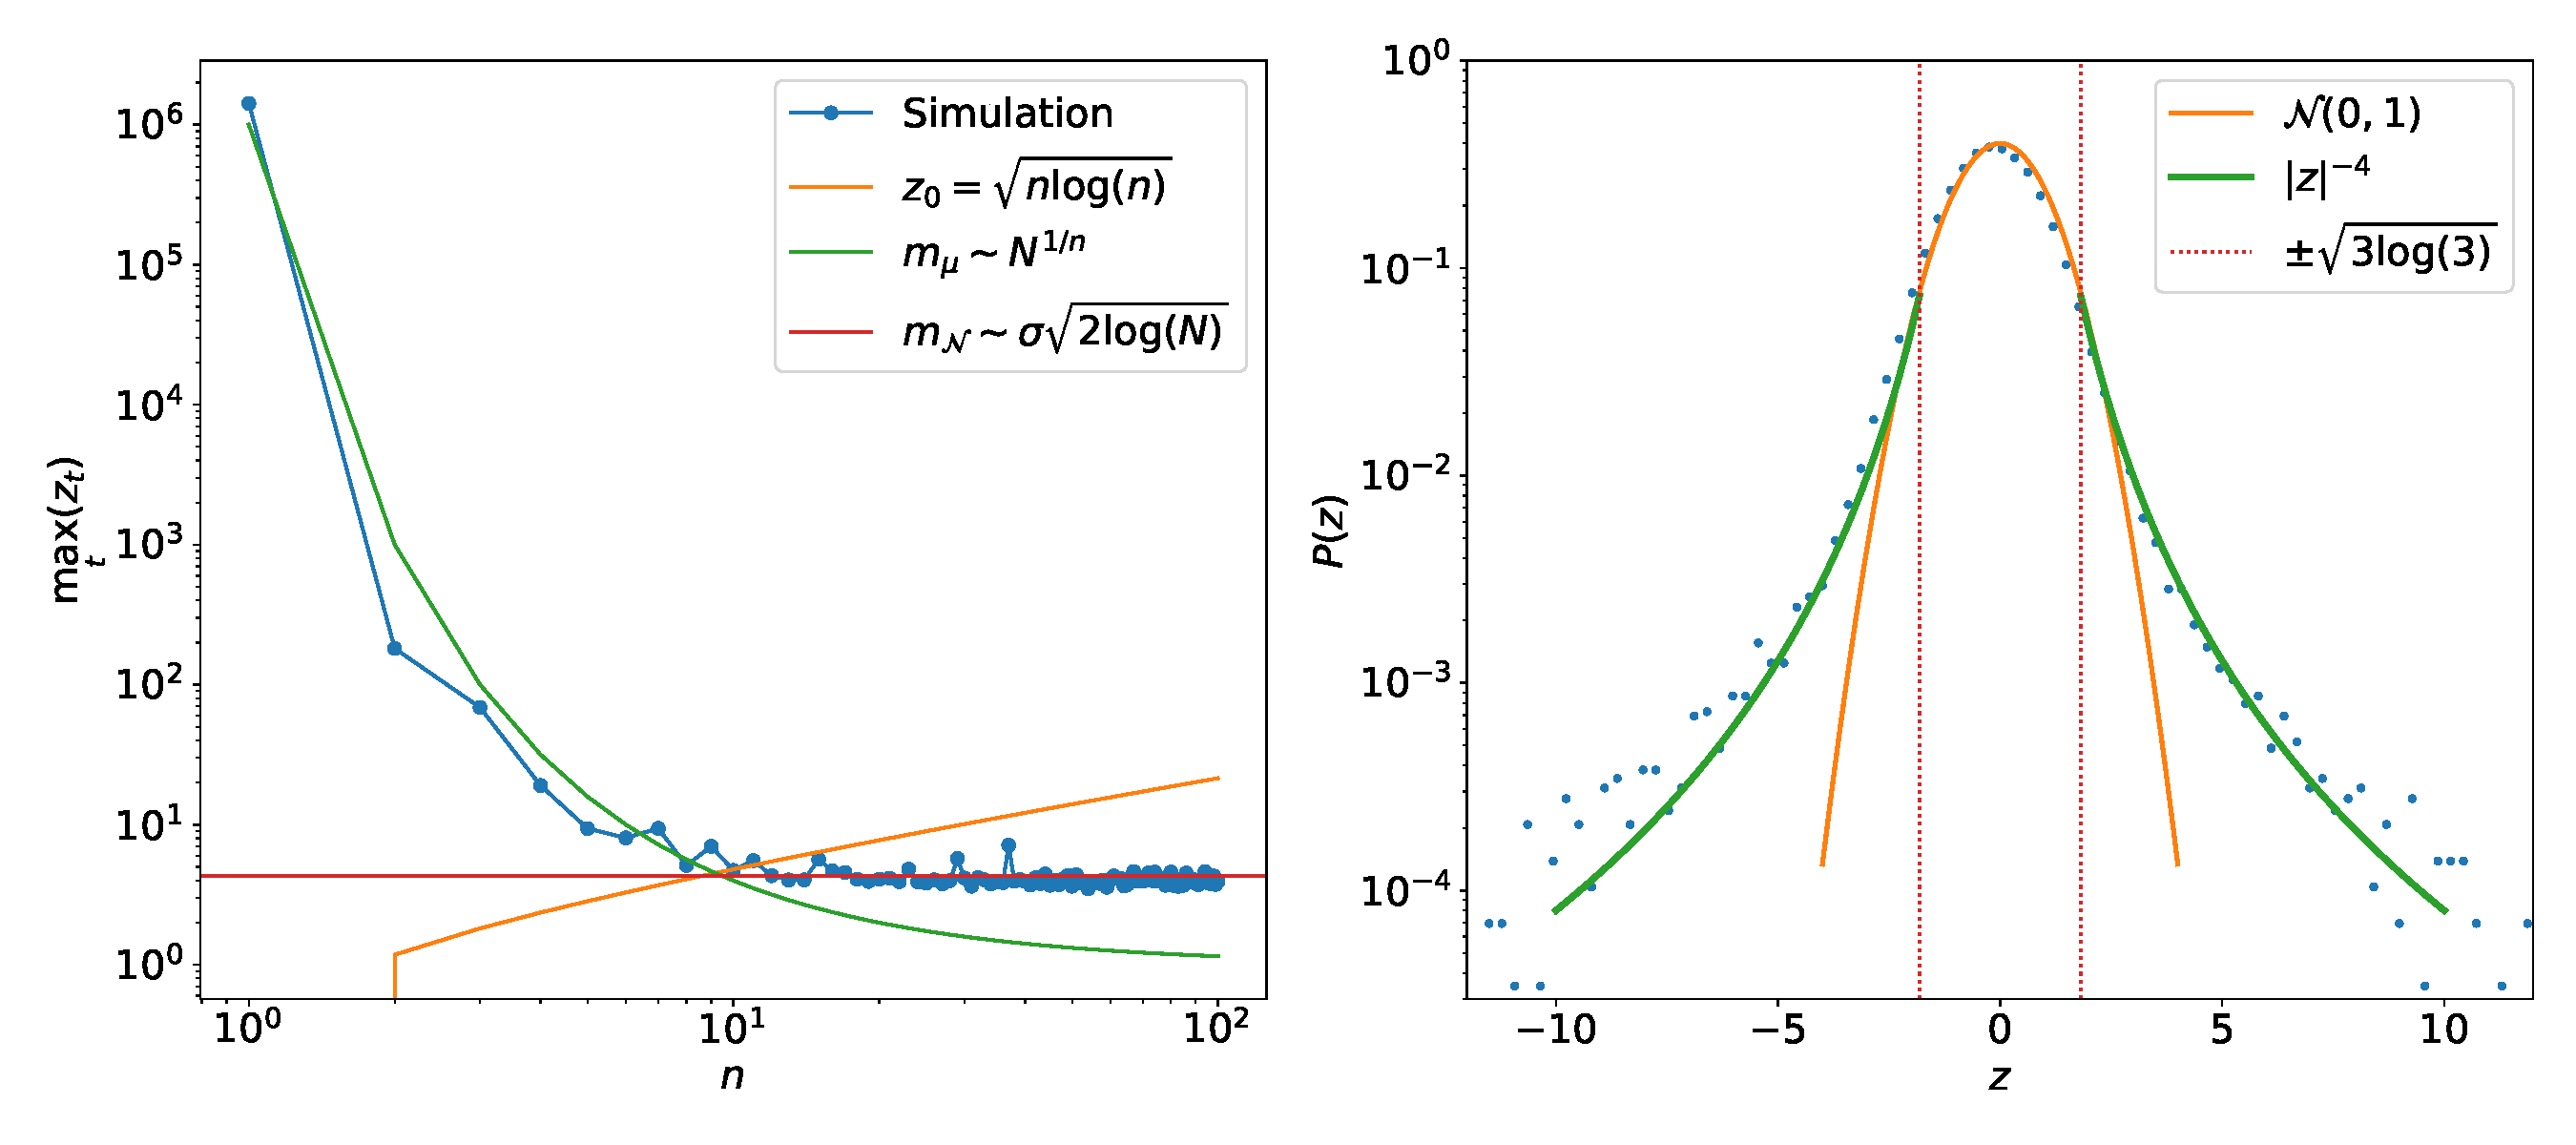
\includegraphics[width=1.1\textwidth ]{Graphs/max_n_hist.pdf}}
	\caption{Left: Convergence of the tail. Maximum value of the time series $z_{max}$ (blue), with trendline for the typical maximum of a sequence of power laws $m_n\sim N^{1/n}$ (green) and normally distributed variables $m_\mathcal{N}\sim \sigma_0\sqrt{2\log(N)}$ (red, \autoref{app:max_distrib} ). Orange line gives the typical threshold beyond which convergence toward a Gaussian is invalid: once $z_{max}<z_0(n)$ the whole distribution becomes normally distributed, without a remaining power tail. Equating $m_\mu(n)=m_\mathcal{N}(n)$ with $N=10^5$ gives the threshold at $n\approx9$, which fits with the observations on both graphs. 
	Right: Illustration of convergence in the centre. Histogram of $z_t$ for $n=3$, with logarithmic $y$ axis. In the region in between $\pm\sqrt{n\log(n)}$ (red borders), $z_t$ follows closely a normal distribution (orange), while the tail still follows a power law $P(z)\sim \abs{z}^{-4}$ after (green).
	$N=10^5$ time-steps, $\alpha_0=2$, $\sigma_0^2=0.8$, $z_0=1$.}
	\label{fig:max_exp_n}
\end{figure}


\end{document}